\documentclass[12pt]{scrartcl}%{report}%{scrbook}%

\usepackage[T1]{fontenc}
\usepackage{amsfonts,amssymb,amsmath,amsthm}
\usepackage[english]{babel}
%\usepackage[ngerman]{babel}
\usepackage[latin1,applemac]{inputenc}
\usepackage{graphicx}
\usepackage{bbm}
\usepackage{dsfont}
\usepackage{caption}
\usepackage{subcaption}
\usepackage{tabularx}
\usepackage{cite}
\usepackage{float}
\usepackage{bigints}
\usepackage[makeroom]{cancel} 
\DeclareMathOperator{\arcsinh}{arcsinh}
\usepackage{hyperref}
\hypersetup{
    colorlinks=true,
    linkcolor=blue,
    filecolor=magenta,      
    urlcolor=cyan,
    pdftitle={Overleaf Example},
    pdfpagemode=FullScreen,
    }

\setlength{\textwidth}{160.0mm}
\setlength{\textheight}{232.0mm}

\renewcommand{\raggedsection}{\centering}


\newtheorem{thm}{Theorem}
\newtheorem{defi}{Definition}
\newtheorem{lem}{Lemma}
\newtheorem{prop}[thm]{Proposition}
\newtheorem{cor}{Corollary}
% \newtheorem{ba}{Proof}
\newtheorem{ex}{Example}
\newtheorem{rem}{Remark}
\title{Sound of Surfaces}
\date{\vspace{-4ex}}

\begin{document}
\maketitle
This app is a software synthesizer that makes virtual surfaces sound.
\section*{Run the App}
\begin{enumerate}
\item Clone the following \href{https://github.com/ChristophSeidel1234/Surface_Sound}{GitHub repository}.
\item This app requires the python modules: \texttt{numpy}, \texttt{scipy}, \texttt{pandas} and \texttt{streamlit}. The first three are standard. If you haven$'$t installed \texttt{streamlit} yet, run\\
\texttt{pip install streamlit}\\
or if you use ANACONDA\\
\texttt{conda install -c conda-forge streamlit}
\item Open a terminal, go to the current working directory and run\\
\texttt{streamlit run app.py}\\ This command will open the app in your preferred browser.
\end{enumerate}

\section*{Instructions}
We go step by step from top to bottom through the app.
\begin{itemize}
\item \textbf{Select Surface}\\
I have chosen the shape of the surfaces (i.e. tuned them) so that the fundamental tone together with the first overtones form a major, minor or power cord.
\begin{figure}[!htb]
\minipage{0.25\textwidth}
  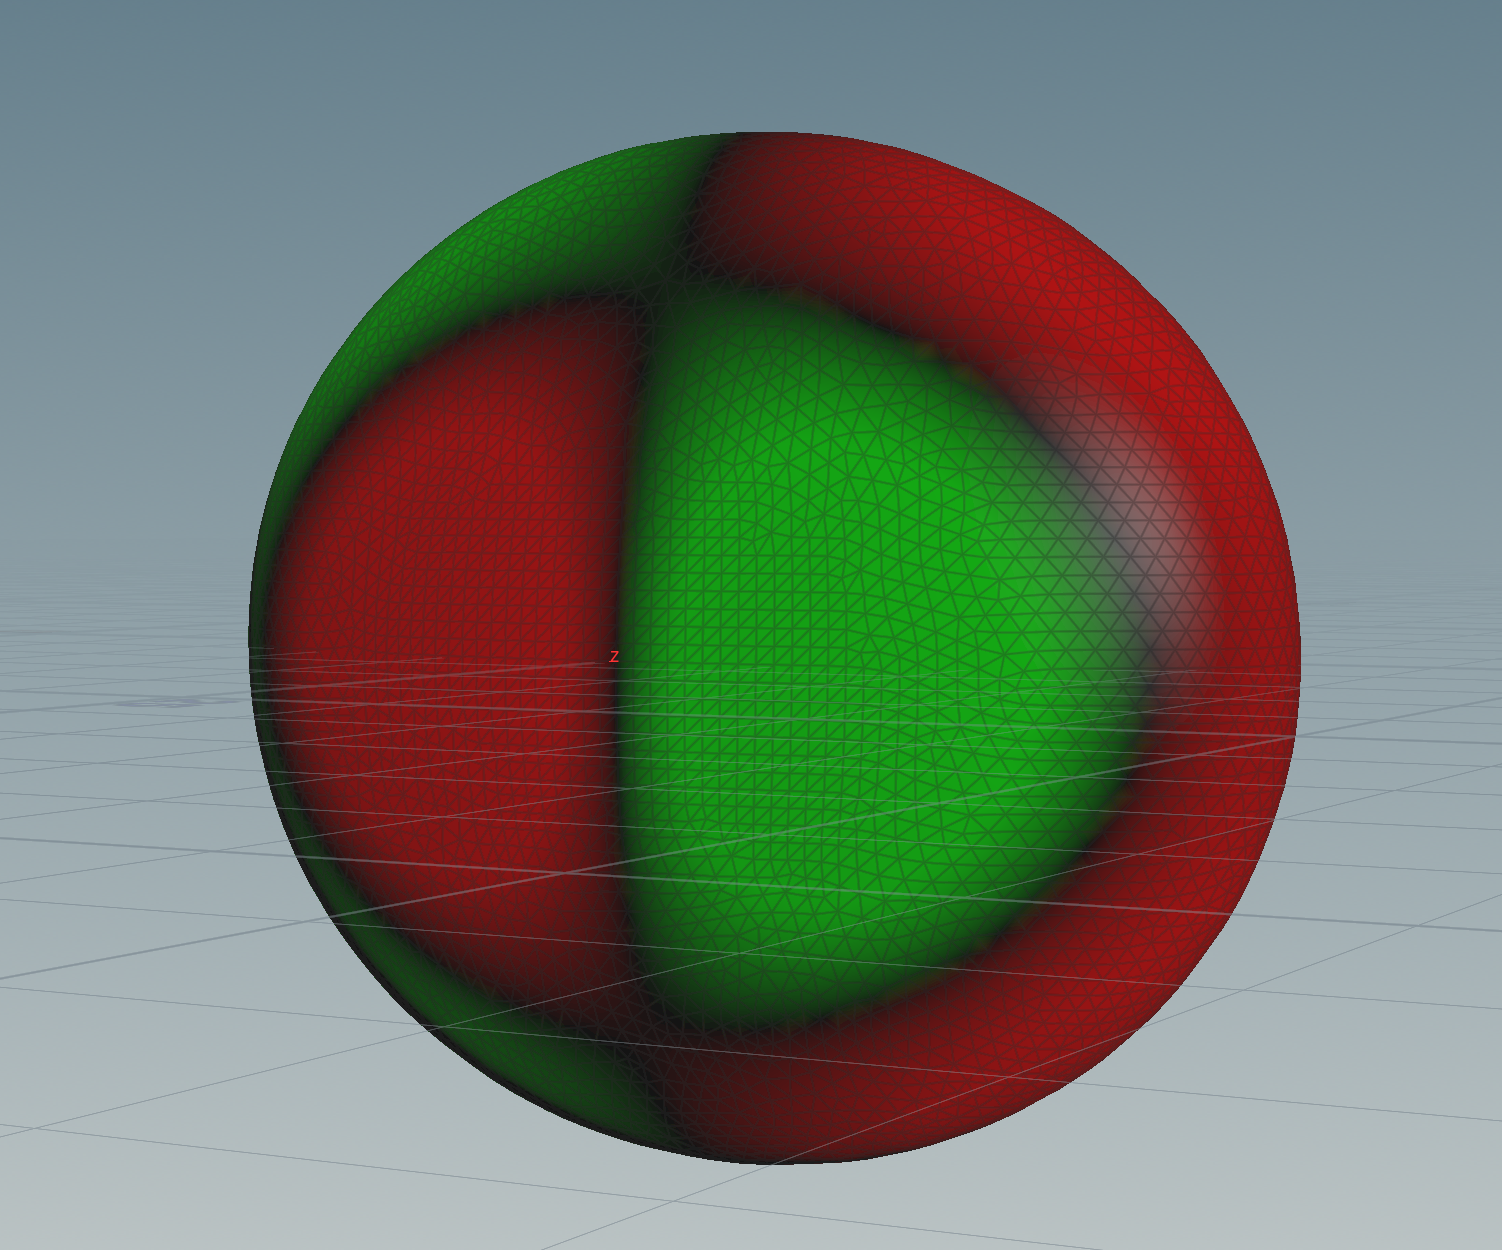
\includegraphics[width=\linewidth]{major}
  \caption{Major Ellipsiod}
\endminipage\hfill
\minipage{0.25\textwidth}
  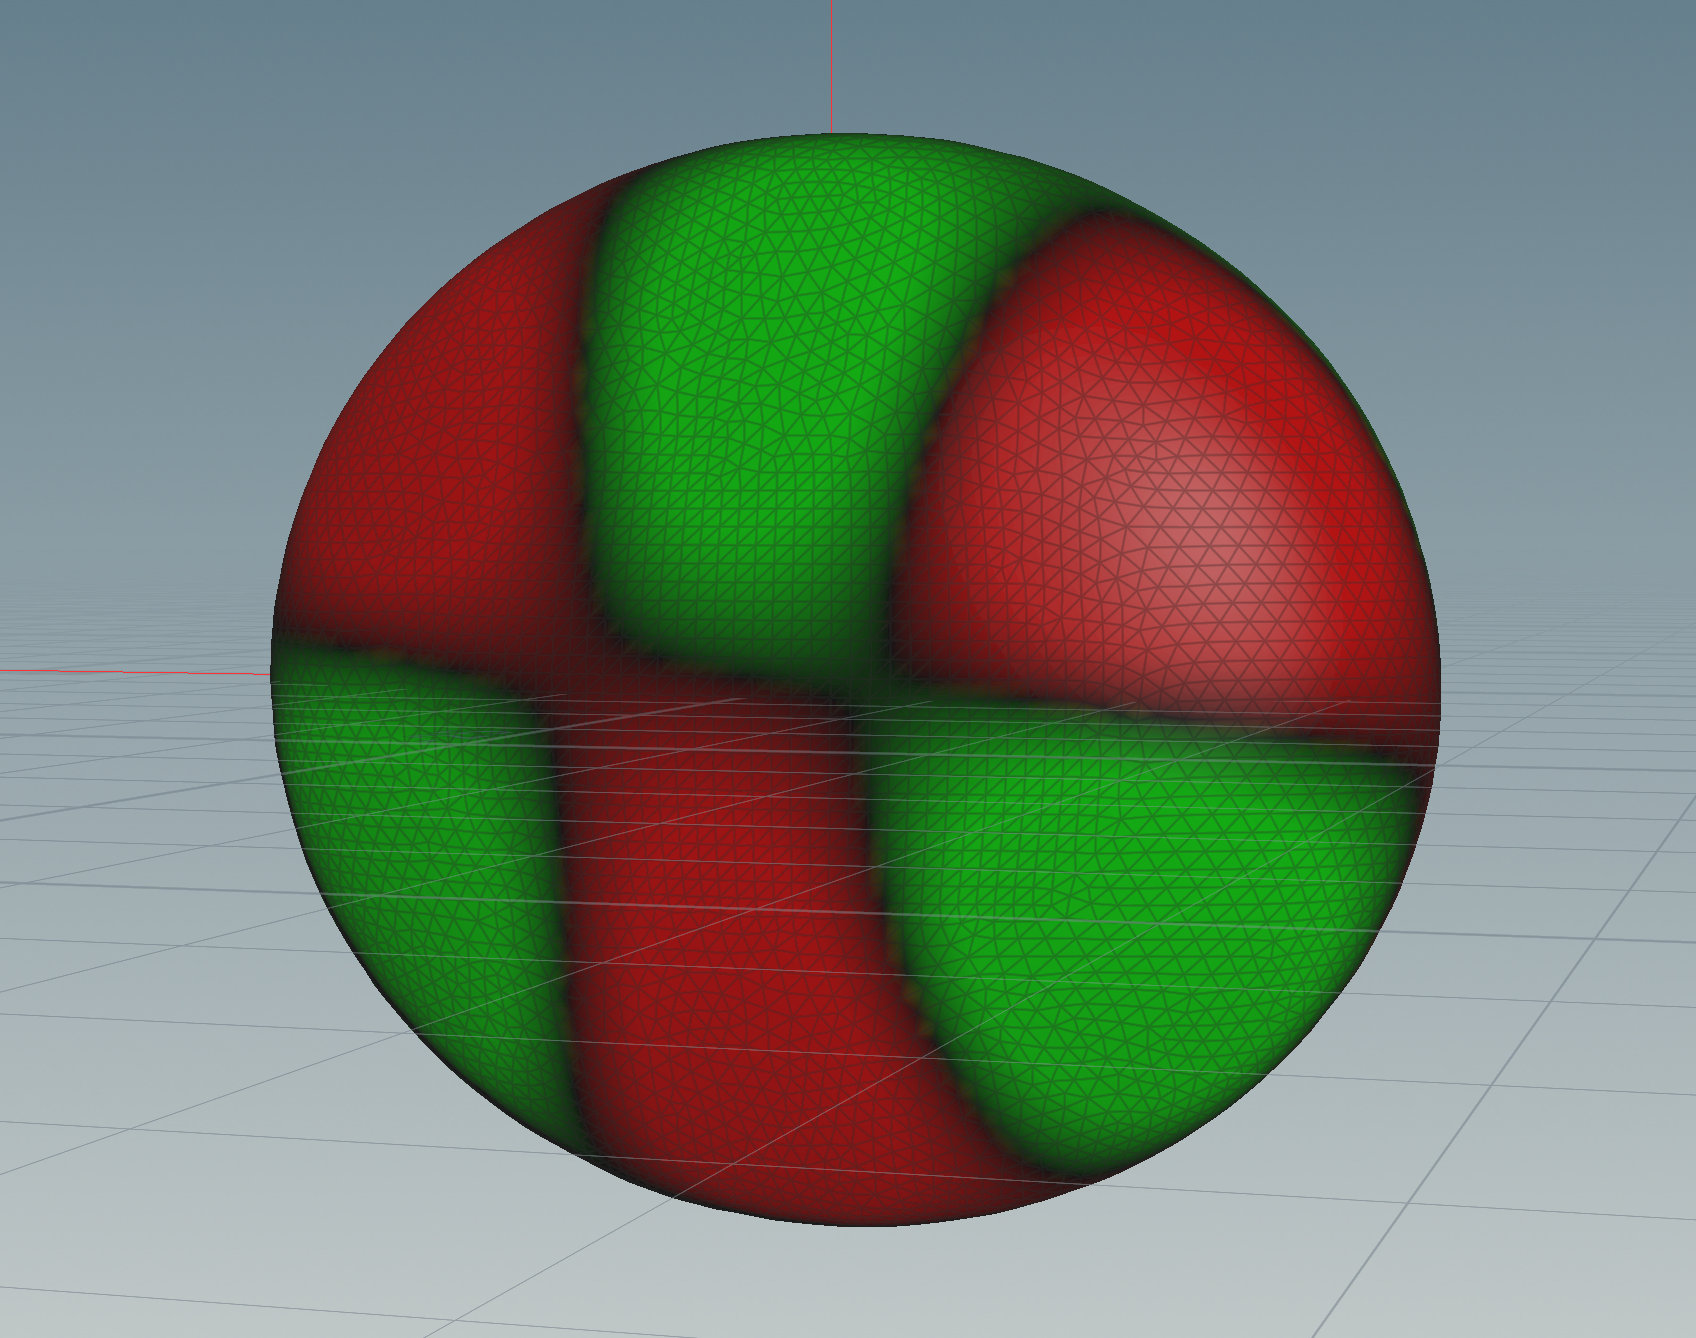
\includegraphics[width=\linewidth]{minor}
  \caption{Minor Ellipsiod}
\endminipage\hfill
\minipage{0.25\textwidth}%
  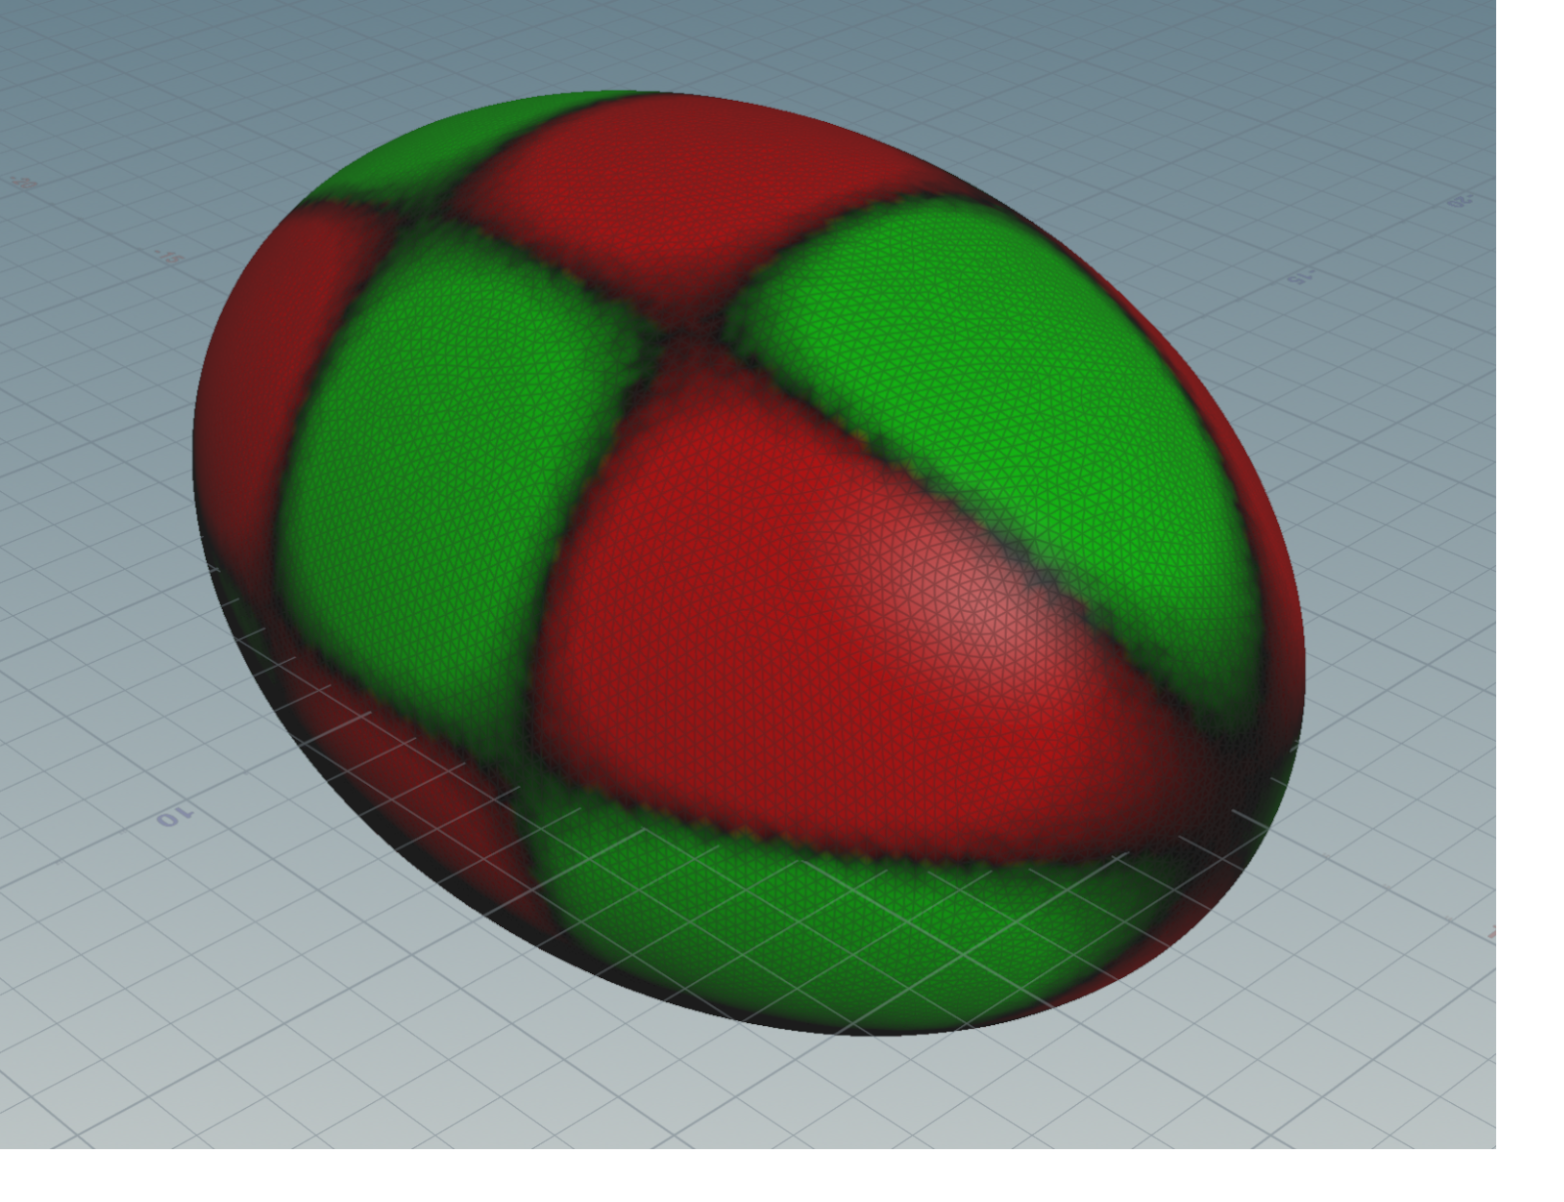
\includegraphics[width=\linewidth]{power}
  \caption{Power Ellipsiod}
\endminipage
\end{figure}
\item \textbf{Number of Overtones}\\
Here you can set the number of generalized harmonics. If you select more, the sound becomes more glassy. 
\item \textbf{Select Waveform}\\
These are the different initial conditions. For example, cone means that one pulls out something like a tent at the surface, comparable with picking a guitar string.
\item \textbf{Pick or Strike}\\
Pick gives the location and strike the speed in the initial conditions. If you think of physical instruments, this would be the difference between a piano and a harpsichord. 
\item \textbf{Propagation Velocity}\\
This means how fast is the speed of the wave on the surface. This is also like tuning an instrument, since the propagation velocity is coupled to the frequencies in the wave equation.

\end{itemize}
\vspace{2cm}
Finally, I would like to mention that each change of the above options writes or changes a file named \texttt{new\_signal.wav} on your desktop with respect to the selected properties.
\end{document}